% Updated from the supplied draft using the project evidence audited on 2026-11-06.
% Build main.tex with pdfLaTeX + BibTeX (Overleaf) or Tectonic.
% See evidence_audit.md and missing_or_unverified.md for verification boundaries.
\documentclass[conference]{IEEEtran}
\IEEEoverridecommandlockouts
\usepackage[T1]{fontenc}
\usepackage[utf8]{inputenc}
\usepackage{amsmath,amssymb,graphicx,booktabs,array}
\usepackage{url,cite}
\usepackage{balance}
\usepackage{tikz}
\usetikzlibrary{arrows.meta,positioning}
\usepackage[hidelinks]{hyperref}
\newcommand{\code}[1]{\texttt{#1}}
\newcommand{\NR}{---}
\newcommand{\ClassRows}{%
0 & air\_conditioner & 1,000 & 100 \\
1 & car\_horn & 429 & 36 \\
2 & children\_playing & 1,000 & 100 \\
3 & dog\_bark & 1,000 & 100 \\
4 & drilling & 1,000 & 100 \\
5 & engine\_idling & 1,000 & 96 \\
6 & gun\_shot & 374 & 35 \\
7 & jackhammer & 1,000 & 120 \\
8 & siren & 929 & 86 \\
9 & street\_music & 1,000 & 100 \\
}

\newcommand{\PerClassRows}{%
0 & 100 & 72.63 & 69.00 & 0.7077 \\
1 & 36 & 87.80 & 100.00 & 0.9351 \\
2 & 100 & 98.00 & 98.00 & 0.9800 \\
3 & 100 & 89.52 & 94.00 & 0.9171 \\
4 & 100 & 98.55 & 68.00 & 0.8047 \\
5 & 96 & 82.29 & 82.29 & 0.8229 \\
6 & 35 & 100.00 & 100.00 & 1.0000 \\
7 & 120 & 77.40 & 94.17 & 0.8496 \\
8 & 86 & 96.63 & 100.00 & 0.9829 \\
9 & 100 & 97.94 & 95.00 & 0.9645 \\
}

\newcommand{\ComparisonRows}{%
head & 20,490 & 87.73 & 0.8638 & 4 & 19.80 & 474.2 \\
fc1 & 4,216,842 & 88.06 & 0.8668 & 4 & 18.87 & 522.3 \\
block6 & 60,848,138 & 90.65 & 0.9010 & 4 & 28.65 & 1278.1 \\
}

\newcommand{\SampleRateRows}{%
8,000 & 12 \\
11,024 & 7 \\
11,025 & 39 \\
16,000 & 45 \\
22,050 & 44 \\
24,000 & 82 \\
32,000 & 4 \\
44,100 & 5,370 \\
48,000 & 2,502 \\
96,000 & 610 \\
192,000 & 17 \\
}

\title{Deep Learning Framework for Environmental Sound Recognition Using PyTorch\\
\large A Single-Fold Study of Selective Fine-Tuning of AudioSet-Pretrained PANNs CNN14}
\author{\IEEEauthorblockN{Ayush Ranjan and Sandeep Gupta}
\IEEEauthorblockA{Department of Data Science and Engineering\\
Manipal University of Jaipur\\Jaipur, India\\
ayushranjan.works@gmail.com}}
\begin{document}
\maketitle

\begin{abstract}
This study examines how the depth of adaptation affects environmental sound classification with an AudioSet-pretrained PANNs CNN14 model. Three configurations train a ten-class linear head alone, the final fully connected layer and head, or the final convolutional block together with those layers. UrbanSound8K's predefined assignments are retained: folds 3--10 provide 6,971 training clips, fold 2 provides 888 validation clips, and fold 1 provides 873 test clips. With a common six-epoch budget and one random seed, the final-block configuration obtains the highest validation macro-F1, 0.9010, at epoch 4. The selected checkpoint correctly classifies 773 test clips, giving 88.55\% accuracy and 0.8964 macro-F1. Its 60,848,138 trainable parameters constitute 74.33\% of the instantiated model. Relative to head-only training, the validation accuracy is 2.93 percentage points higher, with approximately 1.45 times the recorded epoch runtime and 2.70 times the peak allocated GPU memory. These findings describe one split, rather than a ten-fold benchmark. A metadata audit also identifies five source recording IDs shared across predefined folds, limiting source independence. The evidence supports a measured validation performance--cost trade-off; it does not establish statistical superiority, cross-fold stability, or a new state of the art.
\end{abstract}
\begin{IEEEkeywords}
environmental sound classification, UrbanSound8K, PANNs CNN14, AudioSet, PyTorch, transfer learning, selective fine-tuning
\end{IEEEkeywords}

\section{Introduction}\label{sec:intro}
Environmental sound classification assigns categories such as siren, drilling, or dog bark to audio recordings. Variations in recording conditions and similarities between sound sources make this a challenging recognition task. UrbanSound8K provides ten labeled classes and predefined folds for reproducible evaluation \cite{salamon2014urbansound,urbansoundwebsite}. Pretraining on a larger audio collection offers a way to initialize representations before adapting them to these categories. AudioSet supplies broad audio-event annotations \cite{gemmeke2017audioset}, and PANNs provides pretrained networks and their source implementation \cite{kong2020panns,pannsrepo}.

The amount of adaptation is an empirical design choice. Training only a new classification head limits optimization to a small number of weights, whereas unfreezing pretrained layers allows task-specific changes at a higher computational cost. Neither improved generalization nor reduced overfitting follows solely from increasing or decreasing the trainable parameter count.

This paper investigates three questions: (1) how do three freezing depths differ on a common validation partition; (2) how does the validation-selected checkpoint perform on the reserved test fold; and (3) what runtime and memory costs accompany the additional trainable layers? The contribution is a documented freezing-depth experiment using an existing architecture. It comprises three complete training histories, checkpoint-linked test predictions, and a dataset/source-overlap audit. The experiment uses one seed and one test fold, so it cannot answer questions about stability across folds or seeds. Head-only and intermediate-depth test results are unavailable; consequently, the controlled configuration comparison is restricted to validation data.

\section{Prior Work}\label{sec:related}
Piczak \cite{piczak2015cnn} studied a CNN operating on segmented spectrograms and their deltas. The original paper reports 73.1\% mean UrbanSound8K accuracy for its long-segment probability-voting configuration (LP). The nearby 73.7\% value refers to an unsupervised-learning comparator (US), rather than that CNN configuration. Salamon and Bello \cite{salamon2017augmentation} report approximately 73\% mean accuracy without augmentation and 79\% with augmentation for their spectrogram CNN under ten-fold evaluation.

Guzhov \emph{et al.} \cite{guzhov2020esresnet} investigated visual-domain transfer and evaluation protocols. Their Table~II distinguishes ESResNet from ESResNet-Attention: the ImageNet-pretrained attention model achieves 84.21\% with mono input and 85.42\% with stereo input. These are different from the corresponding plain ESResNet results. Their reproducibility analysis also distinguishes official-fold evaluations from results obtained under other split procedures.

Su \emph{et al.} \cite{su2019fusion} proposed two-stream decision fusion. Their reported 97.2\% UrbanSound8K result is not a suitable official-fold benchmark: Guzhov \emph{et al.}'s reimplementation study attributes that work's results to an unofficial split \cite{guzhov2020esresnet}. This is a conclusion of the cited reproducibility study, not a new reproduction performed here.

PANNs uses AudioSet pretraining for audio representations \cite{kong2020panns}. The original CNN14 produces a 2,048-dimensional embedding and 527 sigmoid tagging scores \cite{pannsrepo}. AudioSet tagging and UrbanSound8K single-label classification have different outputs and metrics. We attach a separate ten-class head to the embedding rather than interpreting the AudioSet scores as target-class probabilities.

\section{Dataset and Evaluation Protocol}\label{sec:data}
\subsection{Dataset inspection}
The official UrbanSound8K description specifies 8,732 excerpts of up to four seconds, ten classes, and ten folds \cite{urbansoundwebsite}. Table~\ref{tab:classes} and Fig.~\ref{fig:classes} give counts recomputed from the local metadata; class IDs retain their official meanings. The minority classes make macro-averaged metrics useful alongside accuracy.

\begin{table}[t]
\centering\caption{Verified local class totals and fold-1 test supports.}\label{tab:classes}
\footnotesize\setlength{\tabcolsep}{4pt}
\begin{tabular}{@{}r l r r@{}}\toprule
ID & Official label & All clips & Test clips\\\midrule
\ClassRows
\midrule & Total & 8,732 & 873\\\bottomrule
\end{tabular}
\end{table}

\begin{figure}[t]
\centering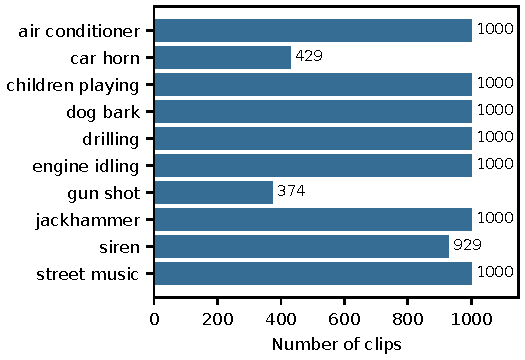
\includegraphics[width=\columnwidth]{figures/class_counts.pdf}
\caption{Class counts calculated from the local UrbanSound8K metadata. These are dataset measurements, not classifier outputs.}\label{fig:classes}
\end{figure}

A preserved full-decoding report records 8,732 successful decodes and no invalid files. A fresh header inspection agrees with its sample-rate, channel, and duration summaries: 7,993 files are stereo and 739 are mono; 5,370 are at 44.1~kHz and 2,502 at 48~kHz. The full range is 8--192~kHz. Header-derived duration has minimum 0.050~s, median 4.000~s, mean 3.6075~s, and maximum 4.03665~s. Eight local files exceed four seconds slightly. Thus, the dataset's nominal duration description must be distinguished from the measured sample-count durations. The preprocessing handles both shorter and longer files. The accompanying dataset README specifies CC BY-NC 3.0 and provides attribution instructions.

\subsection{Partitions and source overlap}
Training uses folds 3--10 (6,971 clips); validation uses fold 2 (888 clips); and testing uses fold 1 (873 clips). File keys, defined by fold and filename, are disjoint across these partitions. The recorded global random seed is 67. Both freezing depth and checkpoint epoch were selected using validation macro-F1. The dated validation review selects \code{block6} at epoch 4; the subsequent evaluation record identifies that checkpoint by its SHA-256 hash.

Maintaining predefined folds does not establish perfect source independence in the local metadata. Five Freesound IDs occur in more than one fold (Table~\ref{tab:overlap}). Four span training and testing; one spans training and validation. In total, 91 of the 873 test clips have source IDs also present in training. Some associated annotated intervals overlap. This dependence can affect evaluation, but the available records do not quantify its effect on accuracy. We preserve the recorded fold assignments and explicitly disclose the issue instead of describing the test data as source-disjoint.

\begin{table}[t]
\centering\caption{Source IDs crossing predefined folds in the local metadata. ``Pairs'' counts cross-fold clip pairs with positive annotated temporal overlap; it is not a count of unique clips.}\label{tab:overlap}
\footnotesize
\begin{tabular}{@{}r c r r@{}}\toprule
Source ID & Folds & Clips (both folds) & Pairs\\\midrule
77751 & 2, 7 & 30 & 31\\
106905 & 1, 8 & 7 & 0\\
132016 & 1, 4 & 15 & 0\\
176638 & 1, 4 & 5 & 1\\
180937 & 1, 9 & 95 & 57\\\bottomrule
\end{tabular}
\end{table}

The dataset authors recommend averaging results across all ten predefined test folds \cite{urbansoundwebsite}. Only fold 1 was evaluated here. The reported accuracy is therefore a single-fold estimate and is not directly comparable to a published ten-fold mean.

\section{Audio Representation and Model Adaptation}\label{sec:model}
\subsection{Waveform preprocessing and CNN14}
The loader reads float32 waveforms, averages channels to mono, and resamples to 32~kHz using \code{librosa} with \code{soxr\_hq} when necessary. It then applies a deterministic center crop or right zero-padding to obtain 128,000 samples (four seconds). There is no per-clip loudness normalization or additional waveform augmentation in the dataset loader. Training, validation, and testing use the same deterministic waveform preparation.

The unchanged upstream \code{Cnn14} implementation computes the spectrogram and log-Mel representation internally. Its configured front end uses a Hann window of 1,024 samples, a hop of 320 samples, 64 Mel bins, and a frequency range of 50--14,000~Hz. These correspond to 32-ms windows and 10-ms hops. Six two-convolution blocks have widths 64, 128, 256, 512, 1,024, and 2,048. Frequency averaging is followed by the sum of temporal maximum and mean pooling, and then the 2,048-unit \code{fc1} layer \cite{pannsrepo}. Fig.~\ref{fig:pipeline} summarizes the implemented path.

\begin{figure*}[t]
\centering
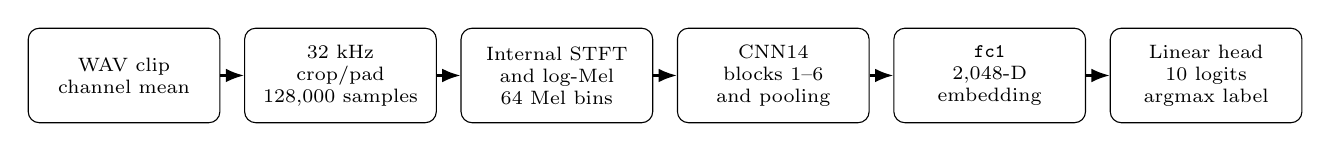
\begin{tikzpicture}[>=Latex,node distance=3mm,
box/.style={draw,rounded corners,align=center,font=\scriptsize,minimum height=12mm,text width=22mm},
flow/.style={-Latex,thick}]
\node[box] (a) {WAV clip\\channel mean};
\node[box,right=of a] (b) {32 kHz\\crop/pad\\128,000 samples};
\node[box,right=of b] (c) {Internal STFT\\and log-Mel\\64 Mel bins};
\node[box,right=of c] (d) {CNN14\\blocks 1--6\\and pooling};
\node[box,right=of d] (e) {\code{fc1}\\2,048-D\\embedding};
\node[box,right=of e] (f) {Linear head\\10 logits\\argmax label};
\draw[flow] (a)--(b);\draw[flow] (b)--(c);\draw[flow] (c)--(d);
\draw[flow] (d)--(e);\draw[flow] (e)--(f);
\end{tikzpicture}
\caption{Implemented downstream path. The original 527-class AudioSet head is retained for checkpoint compatibility but its predictions are unused. The selected configuration trains block 6, \code{fc1}, and the ten-class head; pretrained BatchNorm running statistics stay fixed.}\label{fig:pipeline}
\end{figure*}

The pretrained initialization is \code{Cnn14\_mAP=0.431.pth}, whose MD5 matches the official Zenodo record \cite{pannsweights}. The source is pinned to commit \nolinkurl{d2f4b8c18eab44737fcc0de1248ae21eb43f6aa4}. The model loads the converted tensor-only backbone with strict state-dictionary matching. The original 527-class layer remains present and frozen to preserve compatibility; its output does not contribute to the downstream loss.

\subsection{Ten-class prediction and freezing policy}
Let $f_\theta(x)\in\mathbb{R}^{2048}$ denote the returned embedding. A new affine head produces
\begin{align}
\mathbf{z}_i &= Wf_\theta(x_i)+\mathbf{b}\in\mathbb{R}^{10},\\
p_{ic} &= \frac{\exp(z_{ic})}{\sum_{k=0}^{9}\exp(z_{ik})},\\
\mathcal{L}_{\mathrm{CE}} &=-\frac{1}{B}\sum_{i=1}^{B}\log p_{i,y_i}.
\end{align}
Cross-entropy receives raw logits. Softmax probabilities are used for probability-based evaluation, while the predicted label is the maximum-logit class. The new layer has $2048\times10+10=20,490$ parameters.

Three configurations differ only in the trainable subset: \code{head} trains the new affine head; \code{fc1} additionally trains the pretrained final dense layer; and \code{block6} additionally trains \code{conv\_block6}. The optimizer contains exactly the parameters with \code{requires\_grad=True}. All pretrained BatchNorm running means and variances are held fixed, including those in block 6. The affine BatchNorm parameters of block 6 train when that block is unfrozen.

Freezing weights does not disable stochastic transformations in this implementation. Official CNN14 dropout and SpecAugmentation remain active during training in all three configurations and are disabled during evaluation. SpecAugmentation uses two time stripes with width parameter 64 and two frequency stripes with width parameter 8. Dropout probabilities are 0.2 after convolutional blocks and 0.5 around the final representation path. Mixup is not enabled. Thus, \code{head} is a frozen-weight backbone with training-time augmentation, rather than a cache of deterministic features.

The instantiated model contains 81,857,561 registered parameter elements, including the retained AudioSet head and frozen front-end kernels. Of these, 60,848,138 are trainable in \code{block6} and 21,009,423 are frozen. Parameter counts were checked by reconstructing the model and its freezing policies; they are not estimates taken from a different CNN14 variant.

\begin{table*}[t]
\centering\caption{Controlled comparison on validation fold 2. All runs use seed 67, folds 3--10 for training, six epochs, and the same preprocessing/optimizer settings. Time includes training and validation.}\label{tab:comparison}
\footnotesize\setlength{\tabcolsep}{7pt}
\begin{tabular}{@{}l r r r r r r@{}}\toprule
Configuration & Trainable params & Val. acc. (\%) & Val. macro-F1 & Best epoch & Time (min) & Peak MiB\\\midrule
\ComparisonRows
\bottomrule
\end{tabular}
\end{table*}

\begin{figure*}[t]
\centering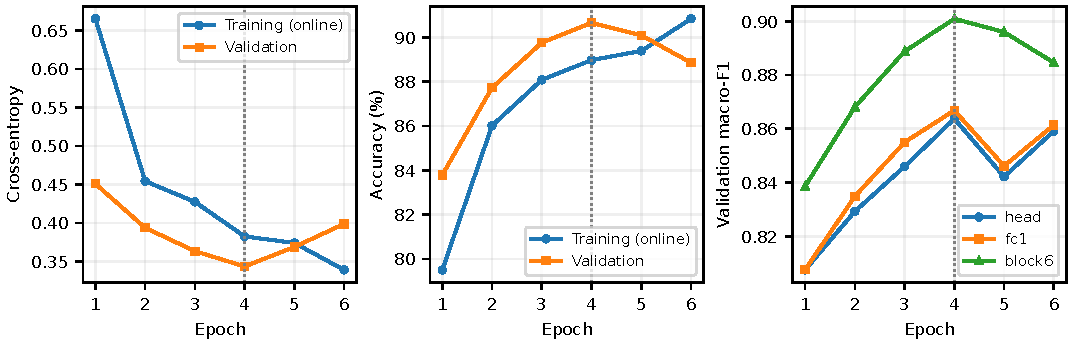
\includegraphics[width=\textwidth]{figures/training_curves.pdf}
\caption{Recorded histories. Left and middle: \code{block6} training/validation loss and accuracy. Right: validation macro-F1 for all three configurations. The dotted line marks selected epoch 4. Online training measurements include dropout and SpecAugmentation, so their difference from evaluation-mode validation metrics is not a controlled generalization-gap estimate.}\label{fig:curves}
\end{figure*}

\section{Training and Measurement}\label{sec:training}
\subsection{Common training settings}
All three complete runs use the settings in Table~\ref{tab:settings}. Six epochs were completed for each configuration, with 6,971 training and 888 validation samples recorded per epoch. The best validation macro-F1 occurs at epoch 4 in every run; accuracy serves as a tie-breaker. Two subsequent epochs without improvement satisfy the recorded patience setting at the six-epoch budget.

\begin{table}[t]
\centering\caption{Settings verified from run configurations and implementation.}\label{tab:settings}
\footnotesize
\begin{tabular}{@{}p{.37\columnwidth}p{.57\columnwidth}@{}}\toprule
Setting & Recorded value / behavior\\\midrule
Optimizer / loss & AdamW / unweighted cross-entropy\\
Head learning rate & $10^{-3}$\\
Trainable backbone rate & $10^{-5}$\\
Weight decay & $10^{-4}$\\
Batch / accumulation & 1 clip / 4 microbatches\\
Epoch budget / patience & 6 / 2\\
Gradient clipping & Maximum norm 1.0\\
Learning-rate scheduler & None\\
Global seed & 67\\
Arithmetic & CUDA BF16 autocast; FP32 loss\\
Checkpoint selection & Validation macro-F1, then accuracy\\
Recorded hardware & RTX 3050 Laptop GPU, 4 GiB\\
Recorded software & Windows 11; Python 3.13.15; PyTorch 2.7.0+cu128\\\bottomrule
\end{tabular}
\end{table}

Gradient accumulation yields 1,743 optimizer steps per epoch; the last accumulation window contains three clips and is scaled accordingly. Historical backward/update diagnostics report unchanged frozen weights and BatchNorm statistics, alongside updates in the intended trainable layers. One diagnostic clip produced zero gradients in later layers, whereas a different training clip produced nonzero gradients. Full histories record nonzero gradients in the monitored head, \code{fc1}, and block-6 weight tensors for every applicable optimizer step. These checks concern monitored tensors, not proof that every trainable scalar changes on every step.

\subsection{Metrics and timing scope}
We report accuracy and macro-averaged precision, recall, and F1 for the ten fixed classes. With confusion counts $C_{ij}$ (true class $i$, predicted class $j$),
\begin{align}
\mathrm{Accuracy}&=\frac{\sum_c C_{cc}}{N},\\
P_c&=\frac{TP_c}{TP_c+FP_c},\qquad
R_c=\frac{TP_c}{TP_c+FN_c},\\
F_{1,\mathrm{macro}}&=\frac{1}{10}\sum_{c=0}^{9}\frac{2P_cR_c}{P_c+R_c}.
\end{align}
Undefined precision/recall/F1 terms use zero. Weighted F1 weights each class F1 by its test support. Specificity is $TN_c/(TN_c+FP_c)$ in a one-versus-rest calculation, then averaged over classes. Macro ROC-AUC averages ten one-versus-rest AUCs computed from saved softmax probabilities; it is not calculated from hard predictions. All classes are represented in the test fold.

Reported runtime is the sum of six recorded epoch timers, each covering training and validation. It excludes initialization and the checkpoint/plot writes that occur outside those timers. Memory is the maximum recorded \code{torch.cuda.max\_memory\_allocated} value, in MiB; it is not total device usage or reserved memory. Each configuration has only one timing observation. No energy or inference-latency measurements are available.

\section{Results}\label{sec:results}
\subsection{Validation comparison and cost}
Table~\ref{tab:comparison} reports the three completed configurations, rather than candidate experiments. The \code{block6} configuration obtains 90.65\% validation accuracy and 0.9010 macro-F1. Relative to \code{head}, the differences are 2.93 percentage points of accuracy and 0.0372 absolute macro-F1; relative to \code{fc1}, they are 2.59 points and 0.0341. These are descriptive differences on the same validation fold used for selection, not held-out estimates of the improvement between models.



For \code{block6}, 74.33\% of registered parameter elements are trainable, compared with 5.15\% for \code{fc1} and 0.025\% for \code{head}. Its epoch runtime is approximately 1.45 times head-only and its peak allocation is 2.70 times head-only. Consequently, the best validation result comes with a substantial adaptation cost. The slightly shorter \code{fc1} runtime than head-only does not establish a speed advantage from a single timing observation.

Fig.~\ref{fig:curves} shows that \code{block6} validation loss increases from 0.3433 at epoch 4 to 0.3986 at epoch 6, while validation macro-F1 falls from 0.9010 to 0.8847. The selected epoch is therefore used for testing. Training loss continues to decrease, but these histories alone do not establish a general overfitting reduction attributable to the freezing policy.

\subsection{Selected-checkpoint test performance}
The saved fold-1 predictions contain one row for every test clip, with matching metadata labels and ten class probabilities. Recalculation yields 773 correct predictions and 100 errors. Aggregate and per-class results appear in Tables~\ref{tab:results} and~\ref{tab:perclass}; the integer confusion matrix is shown in Fig.~\ref{fig:confusion}. These results agree with the preserved evaluation summary. The checkpoint's current SHA-256 matches the evaluation record, and its trainable parameters can be restored into the pinned backbone. This audit recomputes metrics from saved predictions; it does not constitute an independent retraining or a fresh inference replay.

\begin{table}[t]
\centering\caption{Selected \code{block6}, epoch 4, evaluated on fold 1 only ($N=873$). F1 and other nonpercentage metrics use the 0--1 scale.}\label{tab:results}
\footnotesize
\begin{tabular}{@{}l r@{}}\toprule
Metric & Value\\\midrule
Correct predictions & 773 / 873\\
Accuracy & 88.55\%\\
Macro precision & 0.9008\\
Macro recall & 0.9005\\
Macro F1 & 0.8964\\
Weighted precision & 0.8914\\
Weighted recall & 0.8855\\
Weighted F1 & 0.8838\\
Macro specificity (one-versus-rest) & 0.9870\\
Macro ROC-AUC (one-versus-rest) & 0.9909\\
Recorded test cross-entropy & 0.3800\\\bottomrule
\end{tabular}
\end{table}

\begin{table}[t]
\centering\caption{Per-class fold-1 results, recomputed from saved predictions. Class names follow Table~\ref{tab:classes}.}\label{tab:perclass}
\footnotesize\setlength{\tabcolsep}{5pt}
\begin{tabular}{@{}r r r r r@{}}\toprule
ID & Support & Precision (\%) & Recall (\%) & F1\\\midrule
\PerClassRows
\bottomrule
\end{tabular}
\end{table}

\begin{figure}[t]
\centering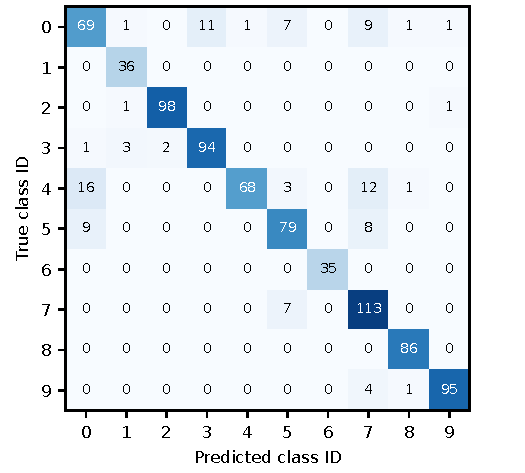
\includegraphics[width=\columnwidth]{figures/confusion_matrix.pdf}
\caption{Fold-1 confusion counts for the selected checkpoint. Rows are true labels and columns are predictions, using the official IDs in Table~\ref{tab:classes}. Counts total 873; the diagonal totals 773.}\label{fig:confusion}
\end{figure}

Drilling and air conditioner have the lowest recalls on this fold, at 68\% and 69\%, respectively. The largest directed error is drilling predicted as air conditioner (16 clips), followed by drilling predicted as jackhammer (12) and air conditioner predicted as dog bark (11). Engine-idling recall is 82.29\%. Car horn, gun shot, and siren each reach 100\% recall on supports of 36, 35, and 86; only gun shot also has 100\% precision. These class-specific results describe the observed fold and do not establish perfect recognition of those sounds in general.

\section{Published Results in Context}\label{sec:published}
Table~\ref{tab:published} provides published context, not a controlled leaderboard. Input representations, pretraining sources, augmentation, and evaluation protocols differ. In particular, this project's fold-1 accuracy cannot be subtracted from ten-fold means to establish superiority. The very high fusion result is explicitly marked as unsuitable for an official-fold comparison.

\begin{table*}[t]
\centering\caption{Published UrbanSound8K results and the scope of this study. Published figures are not project replications.}\label{tab:published}
\footnotesize\setlength{\tabcolsep}{4pt}
\begin{tabular}{@{}p{.25\textwidth}p{.16\textwidth}p{.36\textwidth}r@{}}\toprule
Method & Pretraining & Evaluation / qualification & Accuracy (\%)\\\midrule
Piczak CNN, LP \cite{piczak2015cnn} & None & Ten-fold; original paper's CNN result & 73.1\\
SB-CNN, no augmentation \cite{salamon2017augmentation} & None & Ten predefined folds; rounded original value & $\sim$73\\
SB-CNN, augmentation \cite{salamon2017augmentation} & None & Ten predefined folds; rounded original value & $\sim$79\\
ESResNet-Attention, mono \cite{guzhov2020esresnet} & ImageNet & Official-fold evaluation, Table II & 84.21\\
ESResNet-Attention, stereo \cite{guzhov2020esresnet} & ImageNet & Official-fold evaluation, Table II & 85.42\\
TSCNN-DS \cite{su2019fusion} & Not established here & Reported value; unofficial-split attribution in \cite{guzhov2020esresnet} & 97.2$^\dagger$\\\midrule
This study: CNN14, \code{block6} & AudioSet & One seed; test fold 1; source-overlap caveat & 88.55\\\bottomrule
\end{tabular}
\vspace{1mm}\parbox{.96\textwidth}{\scriptsize $^\dagger$ Retained only as a protocol caution, not an equivalent official-fold benchmark. Piczak's original Section 3 reports LP 73.1\% and US 73.7\%; we use the directly attributed original result despite the 73.70\% Piczak entry in the later ESResNet comparison table.}
\end{table*}

\section{Discussion and Limitations}\label{sec:discussion}
The completed runs support a narrow conclusion: among the three recorded freezing configurations, training block 6 with \code{fc1} and the classifier produced the best validation performance and required more allocated GPU memory and epoch time than head-only training. The reserved-fold result measures the selected model, but does not estimate the held-out gain over the two untested alternatives. Additional unfreezing depths and full fine-tuning were not evaluated in the completed comparison.

Several limitations constrain inference. First, one test fold and one seed cannot characterize fold-to-fold or initialization variance. No confidence interval or significance claim is reported; treating all excerpts as independent would also ignore shared source recordings. Second, source IDs and some annotated intervals cross the retained folds, so strict source independence is not established. The magnitude of any resulting optimism is unknown. Third, validation data serve both configuration and epoch selection, making validation improvements optimistic estimates of a generalizable intervention effect.

Fourth, the evidence audit establishes consistency among stored configurations, predictions, metrics, and checkpoint identity. It does not independently reproduce historical training, verify the historical runtime under repeated trials, or demonstrate that an unrecorded test-driven decision never occurred. The exact project Git revision at training time was not stored in the run configuration; the upstream PANNs commit was. The current audited source revision and file hashes are supplied separately.

Finally, short single-label UrbanSound8K clips do not validate robustness to unseen devices, new locations, long continuous streams, or out-of-taxonomy events. Softmax probabilities are not demonstrated to be calibrated. Cross-dataset duplication between AudioSet pretraining and the target collection has not been audited. No energy efficiency, real-time operation, or deployment readiness claim follows from the current measurements.

\section{Conclusion}\label{sec:conclusion}
This project implements an AudioSet-pretrained CNN14 with a ten-class linear head and compares three freezing depths under a common training protocol. The final-block configuration achieves the highest recorded validation macro-F1, 0.9010, and its epoch-4 checkpoint obtains 88.55\% accuracy and 0.8964 macro-F1 on 873 fold-1 clips. Recomputed metrics, parameter counts, and checkpoint hashes support those recorded values. The associated validation benefit requires substantially more trainable parameters and GPU allocation than head-only training.

The next empirical steps are predefined ten-fold evaluation, repeated seeds, and held-out comparisons of the competing freezing policies. A separately documented source-disjoint sensitivity analysis would address the observed source overlap, while preserving the official-fold results as their own protocol. These experiments remain future work. The present findings should be interpreted as a transparent single-fold study, not a benchmark-wide performance claim.

\appendices
\section{Evidence and Reproduction Notes}\label{app:evidence}
The manuscript audit reads preserved experiment records without retraining or re-evaluating the test audio. The companion \code{audit\_and\_figures.py} recomputes metrics from per-clip predictions, checks labels against metadata, verifies confusion counts, reconstructs the parameter masks, loads the selected checkpoint, and regenerates numerical tables and figures. It also scans local WAV headers. The earlier full-decoding report remains historical evidence rather than a newly repeated decoding test.

The selected training directory is
\begin{quote}\footnotesize
\nolinkurl{results/stage4/20261027_144004_603447_block6_test1}
\end{quote}
and the evaluation directory is
\begin{quote}\footnotesize
\nolinkurl{results/stage5/20261030_132140_664348_block6_test1}.
\end{quote}
The selected checkpoint SHA-256 is
\begin{quote}\footnotesize\ttfamily
7c0e01a0078c225a18f4dc5eaa5110d051\\
ef2c8effec7bcebb4e856e6659328c.
\end{quote}
The line break is for typesetting; the hash is one uninterrupted 64-character value without the final punctuation. The original pretrained file has MD5
\begin{quote}\footnotesize\ttfamily
595633ac2d1cac7ef04ebf70e2fee4e4.
\end{quote}
That MD5 agrees with the official weight release \cite{pannsweights}. The selected checkpoint stores only trainable parameter tensors, not a complete standalone model. Reproduction requires the pinned upstream code and original frozen backbone as well as the selected tensors.

The audit manifest records SHA-256 hashes for the local evidence used in the revision. The audited project revision is
\begin{quote}\footnotesize
\nolinkurl{d5b10c62d086c42ec1f62a70833a0e7916d67b79}.
\end{quote}
This is the revision inspected for the manuscript, not an asserted training-time revision. Saved environment metadata reports \code{torchlibrosa} 0.1.0, \code{librosa} 0.11.0, \code{soundfile} 0.13.1, and scikit-learn 1.7.2. The repository's dependency snapshot is a record of direct package versions rather than a complete transitive lock.

\section{Local Audio Sampling Rates}
Table~\ref{tab:sampling} retains the exact header rates, including 11,024~Hz as distinct from 11,025~Hz. No rate has been rounded into another category. These counts concern original files before conversion to the model's 32-kHz input.
\begin{table}[h]
\centering\caption{Sample rates in all 8,732 local WAV headers.}\label{tab:sampling}
\footnotesize
\begin{tabular}{@{}r r@{}}\toprule
Original sample rate (Hz) & Files\\\midrule
\SampleRateRows
\midrule Total & 8,732\\\bottomrule
\end{tabular}
\end{table}

\section{Selected-Model Parameter Audit}
Table~\ref{tab:parameters} counts registered parameter elements in the reconstructed \code{block6} configuration. BatchNorm running-statistic buffers are not parameters and are excluded from these counts. The spectrogram and log-Mel kernel tensors are registered as frozen parameters in the installed front-end implementation; including them explains part of the difference from a count of learned CNN weights alone.
\begin{table}[h]
\centering\caption{Exact component counts for \code{block6}. F = frozen, T = trainable.}\label{tab:parameters}
\footnotesize\setlength{\tabcolsep}{4pt}
\begin{tabular}{@{}l r c@{}}\toprule
Component & Parameters & Status\\\midrule
Spectrogram extractor & 1,050,624 & F\\
Log-Mel extractor & 32,832 & F\\
\code{bn0} & 128 & F\\
\code{conv\_block1} & 37,696 & F\\
\code{conv\_block2} & 221,696 & F\\
\code{conv\_block3} & 885,760 & F\\
\code{conv\_block4} & 3,540,992 & F\\
\code{conv\_block5} & 14,159,872 & F\\
\code{conv\_block6} & 56,631,296 & T\\
\code{fc1} & 4,196,352 & T\\
\code{fc\_audioset} & 1,079,823 & F\\
Ten-class classifier & 20,490 & T\\\midrule
Total & 81,857,561 & \\
Trainable & 60,848,138 & \\
Frozen & 21,009,423 & \\\bottomrule
\end{tabular}
\end{table}

\section{Measurements Not Available}
No completed ten-fold evaluation, repeated-seed study, test evaluation of \code{head}/\code{fc1}, or full-fine-tuning comparison is present in the final experiment record. Inference latency, energy use, calibration assessment, and out-of-distribution testing are also unavailable. These omissions prevent claims of statistically established improvements, benchmark-wide robustness, or deployment efficiency. They are not represented by fabricated estimates or by substituting results from another dataset.

\balance
\bibliographystyle{IEEEtran}
\bibliography{references}
\end{document}
